\chapter{Partie 1} % Depth 0

\section{Contrainte Budgétaire} % Depth 1

Modèle économique du consommateur : suppose que les individus choisissent ce qu'il y a de meilleur parmi ce qu'ils peuvent acquérir $\Rightarrow$ les consommateurs choisissent le panier qu'ils préfèrent dans leur ensemble budgétaire.
\begin{itemize}
\item[$\rightarrow$] un consommateur ne peut pas dépenser plus que sa richesse. Ce qu'il dépense = quantités qu'il achète $*$ le prix.
\item[$\rightarrow$] Il n'y a pas de place pour effectuer des prêts ou économiser de l'argent.
\end{itemize}

\textbf{La richesse du consommateur est :}
\begin{itemize}
\item soit une richesse exogène (en dehors) au modèle
\item soit la valeur de son panier initial
\end{itemize}

\subsection{Ensemble budgétaire} % Depth 2

L'ensemble budgétaire correspond à l'ensemble de paniers de biens que le consommateur peut s'offrir.

La contrainte budgétaire correspond à la relation :
\begin{equation*}
p_1 x_1 + p_2 x_2 \leq m
\end{equation*}

C'est une inégalité car les paniers accessibles au consommateur sont ceux dont le coût est inférieur ou égal à $m$. Sa pente est de $-\frac{p_1}{p_2}$, son ordonnée à l'origine est à $\frac{m}{p_2}$ et son abscisse à $\frac{m}{p_1}$.

\begin{figure}[H]
    \centering
    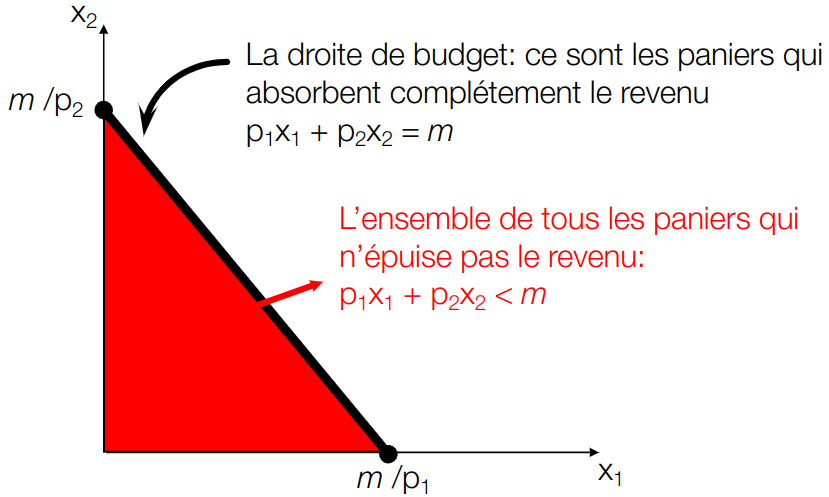
\includegraphics[width=0.4\textwidth,keepaspectratio]{contrainte_budgetaire}
\end{figure}

\subsection{Pente de la droite de budget}

Elle a une représentation économique intéressante : elle mesure le coût d’opportunité de la consommation du bien 1 (taux auquel le consommateur est prêt à substituer le bien 1 au bien 2).
\begin{itemize}
\item[$\rightarrow$] Pour consommer une unité supplémentaire de bien 1, il faut renoncer à $\frac{p_1}{p_2}$ unités de bien 2.
\end{itemize}

\subsection{Déplacement de la droite de budget}

\subsubsection{Variation du revenu}
Déplacement parallèle vers le haut si $m \nearrow$, vers le bas si $m \searrow$

\subsubsection{Variation des prix}
Si $p_1$ diminue, la pente diminue et inversement.

\newpage
\section{Préférences}

\textbf{Panier de biens} : ensemble composé d'un ou de plusieurs produits, représentés par un vecteur $X = (x_1, x_2)$ indiquant la quantité de chacun de ces biens et services.

\textbf{Préférences} : caractérisent comment chaque individu ordonne les alternatives (panier) possibles.
On peut :
\begin{itemize}
\item Préférer strictement $a$ à $b$ (ou l'inverse) : $a \succ b$ ($a \prec b$)
\item Être indifférent entre $a$ et $b$ : $a \sim b$
\item Préférer faiblement $a$ à $b$ (ou l'inverse) : $a \succeq b$ ($a \preceq b$)
\end{itemize}

\subsection{Hypothèse sur les relations de préférences}

\begin{enumerate}
\item \textblue{Complètes} : le consommateur est toujours capable de faire un choix entre 2 paniers
\item \textblue{Réflexives} : tout panier $X$ est au moins aussi désirable que lui-même
\item \textblue{Transitives} : si $a \succeq b$ et $b \succeq c$, alors $a \succeq c$ 
\item \textblue{Monotones} : si par rapport à un panier $Y$, un panier $X$ a une quantité plus importante d'au moins un bien et pas moins de l'autre bien, les pentes des Courbes d'Indifférences (\textit{CI}) seront négatives, et :
	\begin{itemize}
	\item $X \succeq Y$ si les préférences sont faiblement monotones
	\item $X \succ Y$ si les différences sont strictement monotones
	\end{itemize}
\item \textblue{Convexes} : les consommateurs apprécient la diversité et ils préfèrent les paniers intermédiaires aux paniers extrêmes.
\end{enumerate}
$\Longrightarrow$ les préférences normales respectent ces 5 hypothèses.

\subsection{Courbes d'indifférences}

La CI passant par un panier $X$ est composée de tous les paniers laissant le consommateur indifférent à ce panier $X$.

Un panier situé sur une CI plus élevée qu'un autre est strictement préféré à ce dernier $\rightarrow$ deux CI ne peuvent donc pas se croiser.

Graphiquement, si on prend 2 paniers $X$ et $Y$ ($X \sim Y$), toutes les combinaisons convexes de $X$ et $Y$ sont situées sur le segment de droite $[X, Y]$. La convexité des préférences implique que : 
\begin{itemize}
\item Aucun point de ce segment ne se trouve sous la courbe d'indifférence (la CI ne peut dont être une droite).
\item Si la convexité est stricte : tout le segment de droite se situe au-dessus de la CI passant par $X$ et $Y$. Les CI sont alors nécessairement convexes par rapport à l'origine.
\end{itemize}

\subsection{Exemples de préférences}

\subsubsection{Substituts parfaits}

Disposé à substituer un bien par l’autre à un taux constant. La pente vaut -1.
\begin{figure}[H]
	\centering
	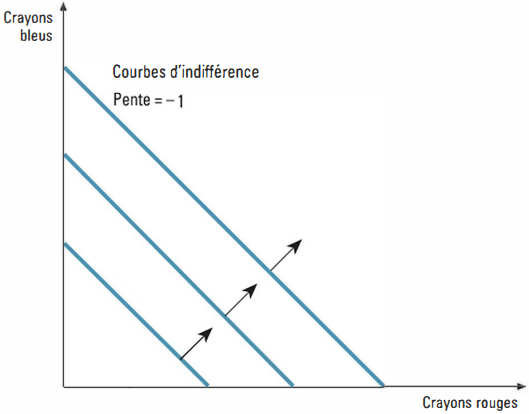
\includegraphics[width=0.4\textwidth,keepaspectratio]{subsituts_parfaits}
\end{figure}

\subsubsection{Compléments parfaits}

Toujours consommés dans des proportions fixes.
\begin{figure}[H]
	\centering
	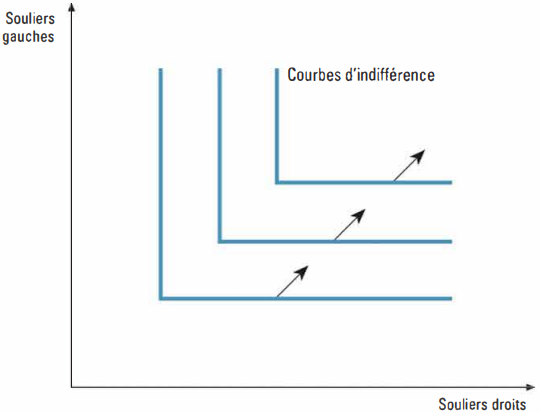
\includegraphics[width=0.4\textwidth,keepaspectratio]{complements_parfaits}
\end{figure}


\subsubsection{Biens indésirables}

Prenons un point $(x_1, x_2)$, un certain nombre de poivrons et d’anchois.

Si nous donnons au consommateur quelques anchois supplémentaires, comment devons-nous modifier la quantité de poivrons pour maintenir le consommateur sur la même CI ? Nous devons lui en donner quelques-uns en plus en échange des anchois supplémentaires. La pente est positive.

\begin{figure}[H]
	\centering
	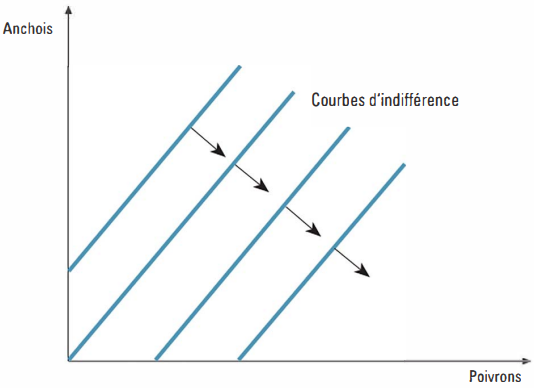
\includegraphics[width=0.4\textwidth,keepaspectratio]{biens_indesirables}
\end{figure}

\subsubsection{Bien neutre}

Le consommateur ne se préoccupe pas du tout du bien 2 (anchois).
\begin{figure}[H]
	\centering
	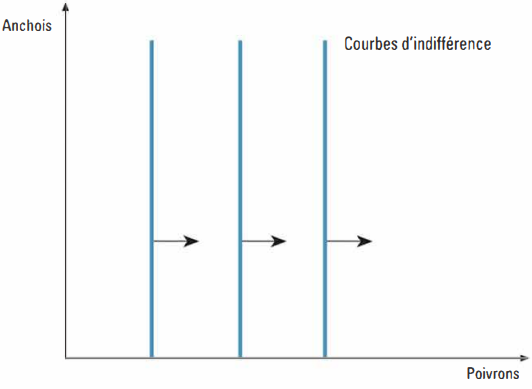
\includegraphics[width=0.4\textwidth,keepaspectratio]{bien_neutre}
\end{figure}

\newpage
\subsubsection{Saturation}

Un point $(x_1,x_2)$ est strictement préféré à tous les autres → plus on s’en éloigne, moins on est satisfait.
\begin{figure}[H]
	\centering
	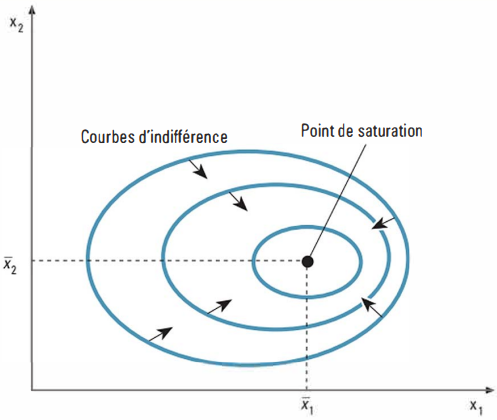
\includegraphics[width=0.4\textwidth,keepaspectratio]{saturation}
\end{figure}

\subsection{Taux Marginal de Substitution (TmS)}

Le TmS mesure la pente de la courbe d'indifférence : $\frac{\Delta x_2}{\Delta x_1}$. Il représente le taux pour lequel le consommateur est indifférent à une substitution de bien 1 au bien 2 (mesure la propension marginale à payer).

\section{L'Utilité}

L'utilité sert à représenter l'ordre dans lequel le consommateur classe les différentes alternatives en fonction de ses préférences.

\begin{enumerate}
\item \textblue{Utilité ordinale} : utilisée ici car on ne se préoccupe que de l'ordre, du classement des préférences. Les valeurs numériques des niveaux d'utilité n'ont pas de signification intrinsèque.
\item \textblue{Utilité cardinale} : la grandeur de l'écart entre les niveaux d'utilité est censée avoir une certaine signification.
\end{enumerate}

\subsection{Fonction d'utilité}

Elle associe à chaque panier une valeur réelle de sorte que si $X \succ Y$, la valeur associée à $X$ ($u(X)$) $>$ à celle associée à $Y$ ($u(Y)$).

Le taux de variation de$f(u)$ peut être mesurée par : $\frac{f(u_1)-f(u_2)}{u_1 - u_2}$. Il sera toujours positif étant donné que le dénominateur auront toujours le même signe.

\subsection{Déterminer les CI à partir d'une fonction d'utilité}

Les paniers situés sur la même Ci ont la même valeur et ceux situés sur des CI supérieures auront des valeurs plus élevées (seul les préférences normales peuvent être représentées par une fonction d'utilité).

\textbf{CI} = ensemble de valeurs $x_1$ et $x_2$ telles que $k = x_1 + x_2$.

\subsection{Exemples de fonctions d'utilité}

\begin{itemize}
\item \textblue{Substituts parfaits} : $u(x_1,x_2) = ax_1 + bx_2$
\item \textblue{Compléments parfaits} : $u(x_1,x_2) = min\{x_1,x_2\}$
\item \textblue{Préférences quasi-linéaires} : $u(x_1,x_2) = f(x_1) + x_2$
\item \textblue{Préférences de Cobb-Douglas} : $u(x_1,x_2) = Ax^c_1x^d_2$ avec $c,d > 0$.
Ici, les CI sont strictement monotones et strictement convexes. Il est toujours possible de trouver une transformation monotone de la fonction qui rende la somme $c+d=1$.
\end{itemize}

\subsection{Utilité marginale}

Variation d'utilité de l'individu lorsqu'il reçoit un peu plus du bien $i$
\begin{equation*}
Um_i = \frac{\Delta u}{\Delta x_i} = \frac{\partial u}{\partial x_i}
\end{equation*}

On peut utiliser la fonction d'utilité pour mesurer le TmS :
\begin{equation*}
TmS = -\frac{Um_1}{Um_2}
\end{equation*}

\section{Le choix}

\textbf{Le choix optimal} : point de tangence entre la CI la plus haute et la droite de budget.
\begin{equation*}
|TmS(x^*_1,x^*_2)| = \frac{p_1}{p_2}
\end{equation*}
\begin{figure}[H]
	\centering
	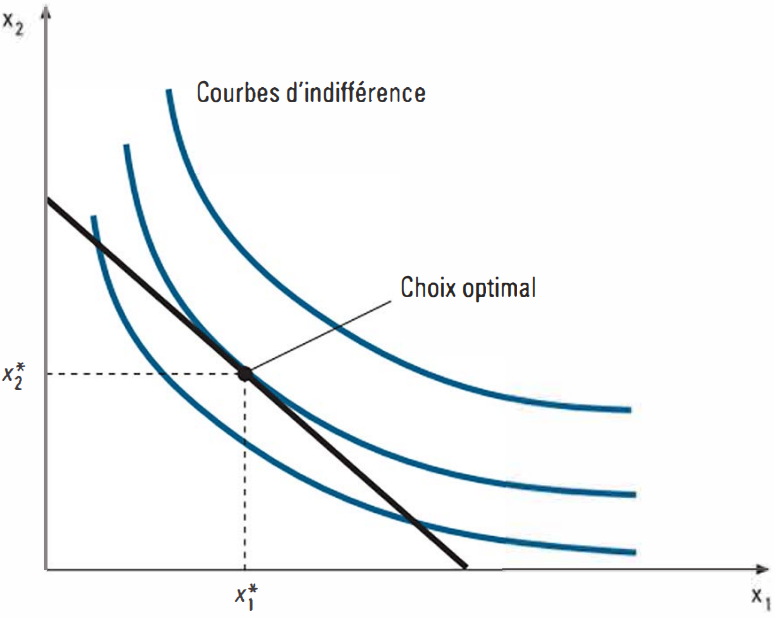
\includegraphics[width=0.4\textwidth,keepaspectratio]{choix_optimal}
\end{figure}

\subsection{2 types de solutions}

\begin{enumerate}
\item Solution intérieure : si $x^*_1 > 0$ et $x^*_2 > 0$, le choix de ($x^*_1,x^*_2$) épuise complètement le budget.
\item Solution de coin : la consommation d'un des biens est nulle.
\end{enumerate}

\subsection{La demande du consommateur}

Panier demandé par le consommateur = quantités optimales de biens 1 et 2. Les fonctions de demande dépendent des prix et du revenu :
\begin{equation*}
x_1(p_1,p_2,m) \text{ } x_2(p_1,p_2,m)
\end{equation*}

\subsection{Fonctions de demande}

\subsubsection{Cobb-Douglas}
\begin{equation*}
x^*_1(p_1,p_2,m) = \frac{am}{(a+b)p_1}
\end{equation*}

\subsubsection{Compléments parfaits}
\begin{equation*}
x^*_1 = x^*_2 = \frac{m}{p_1+p_2}
\end{equation*}

\subsubsection{Substituts parfaits}

\begin{equation*}
x^*_1(p_1,p_2,m) =
\begin{cases}
	0 &\text{ si } p_1 > p_2\\
	[0, \frac{m}{p_1}] &\text{ si } p_1 = p_2\\
	\frac{m}{p_1} &\text{ si } p_1 < p_2
\end{cases}
\text{, }
x^*_2(p_1,p_2,m) =
\begin{cases}
	0 &\text{ si } p_1 < p_2\\
	[0, \frac{m}{p_2}] &\text{ si } p_1 = p_2\\
	\frac{m}{p_2} &\text{ si } p_1 > p_2
\end{cases}
\end{equation*}

\subsubsection{Préférences quasi-linéaires}

Utiliser le Lagrangien ou :
\begin{enumerate}
\item Résoudre une solution intérieure avec $TmS = \frac{p_1}{p_2}$ pour le bien 1 ou 2
\item Trouver la solution pour l'autre bien avec la contrainte de budget
\item Pour avoir une solution intérieure, les deux doivent être > 0 $\rightarrow$ en déduire si c'est une solution de coin ou intérieure (si $\frac{Um_1}{p_1} > \frac{Um_2}{p_2}, x_1 > 0$ et $x_2 = 0$
\item Si c'est une solution de coin :
\begin{itemize}
\item Pour le bien 1 : $(\frac{m}{p_1}, 0)$
\item Pour le bien 2 : $(0, \frac{m}{p_2})$
\end{itemize}
\end{enumerate}

\subsubsection{Conclusion}

\begin{itemize}
\item La contrainte de budget sera toujours effective
\item Le consommateur préfère toujours consommer davantage, il dépense l'intégralité de $m$
\item La demande est homogène de degré 0 : lorsqu'on multiplie tous les prix et le revenue par une constante $t > 0$, la demande ne change pas
\end{itemize}

\section{La demande}

\textbf{Statique comparative} : étudier comment un choix se modifie suite à un changement dans l'environnement économique.

\subsection{Modification du revenu}

\subsubsection{Chemin d'expansion du revenu}

Droite/courbe reliant les paniers demandés à chaque niveau de revenu

\begin{figure}[H]
	\centering
	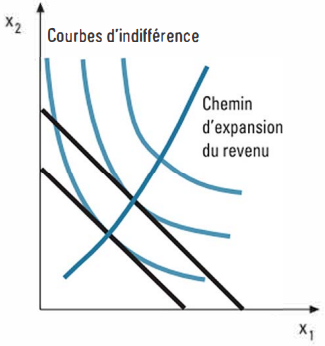
\includegraphics[width=0.27\textwidth,keepaspectratio]{chemin_expansion_revenu}
\end{figure}

\subsubsection{Courbe d'Engel}

Représentation de la demande d'un des biens en fonction du revenu avec les prix constants (revient à isoler $m$)

\begin{figure}[H]
	\centering
	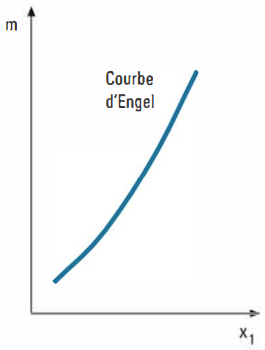
\includegraphics[width=0.24\textwidth,keepaspectratio]{courbe_engel}
\end{figure}

\subsection{Types de biens}

\begin{itemize}
\item  Bien normal : sa demande $\nearrow$ si $m$ $\nearrow$ et inversement. Donc $\frac{\Delta x}{\Delta m} > 0$
\item Bien inférieur : sa demande $\searrow$ si $m$ $\nearrow$. Donc $\frac{\Delta x}{\Delta m} < 0$
\end{itemize}

\begin{minipage}{0.48\textwidth}
	\begin{figure}[H]
		\centering
		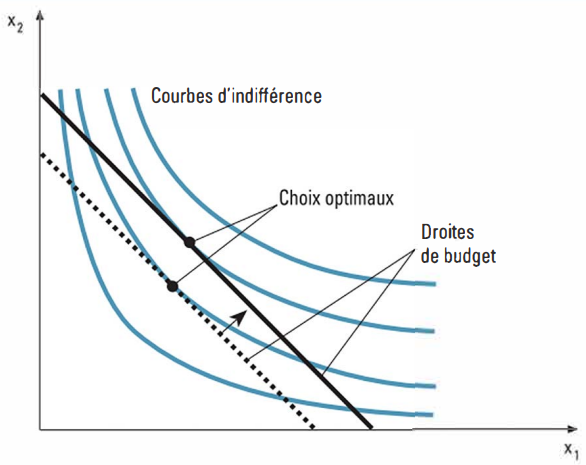
\includegraphics[width=0.8\textwidth,keepaspectratio]{biens_normaux}
		\legend{Biens normaux}
	\end{figure}
\end{minipage}
\begin{minipage}{0.5\textwidth}
	\begin{figure}[H]
		\centering
		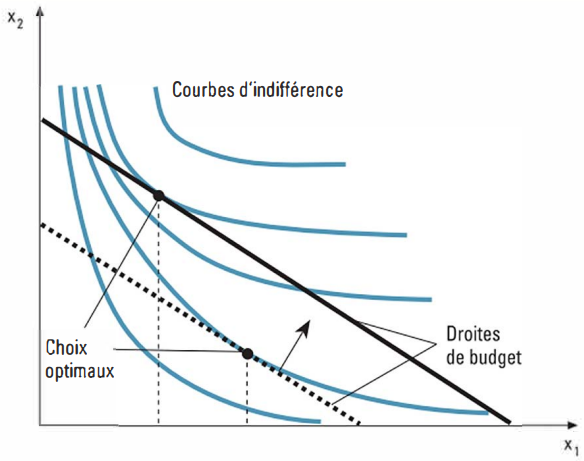
\includegraphics[width=0.8\textwidth,keepaspectratio]{bien_inferieur}
		\legend{Bien inférieur}
	\end{figure}
\end{minipage}

\subsection{Exemples}

\subsubsection{Substituts parfaits}

Ici pour $p_1 < p_2$ (inverse si $p_1 > p_2$)
\begin{figure}[H]
	\centering
	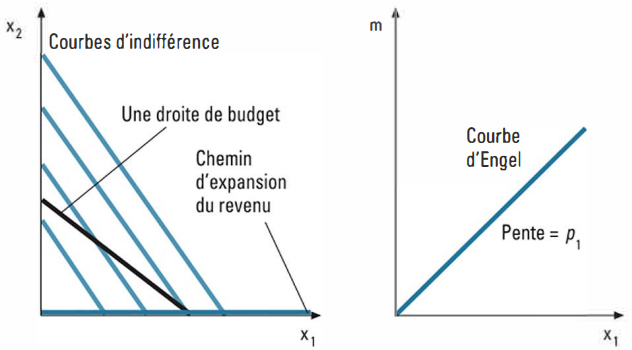
\includegraphics[width=0.5\textwidth,keepaspectratio]{substituts_parfaits_expansion}
\end{figure}

\subsubsection{Compléments parfaits}

\begin{figure}[H]
	\centering
	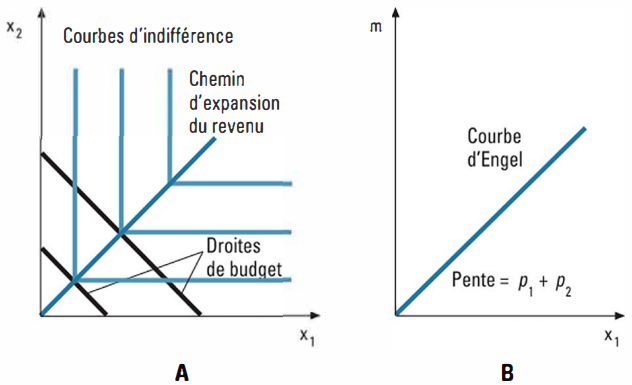
\includegraphics[width=0.5\textwidth,keepaspectratio]{complements_parfaits_expansion}
\end{figure}

\subsubsection{Cobb-Douglas}

\begin{figure}[H]
	\centering
	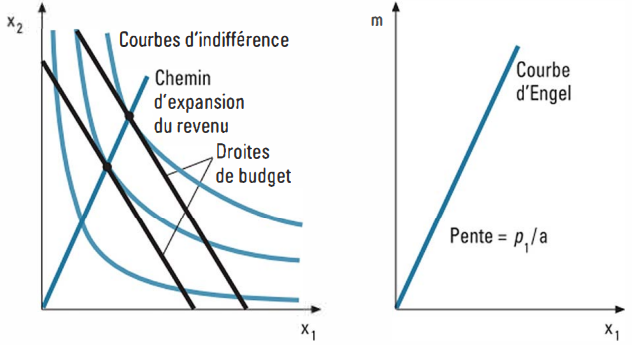
\includegraphics[width=0.5\textwidth,keepaspectratio]{preference_cobb_douglas}
\end{figure}

\subsubsection{Préférences homothétiques}

Biens dont la demande croît dans la même proportion que le revenu. Les substituts parfaits, les compléments parfaits et les préférences de Cobb-Douglas en font partie. Le chemin d'expansion du revenu est alors une ligne droite partant de l'origine.

\paragraph{Bien de luxe}

La demande croît proportionnellement plus que le revenu

\paragraph{Bien de nécessité}

La demande croît proportionnellement moins que le revenu

\subsubsection{Préférences quasi-linéaires}

Elles ne sont pas homothétiques. Le revenu augmente mais la quantité de bien 1 reste la même et tout le revenu supplémentaire est dépensé en bien 2.

\begin{figure}[H]
	\centering
	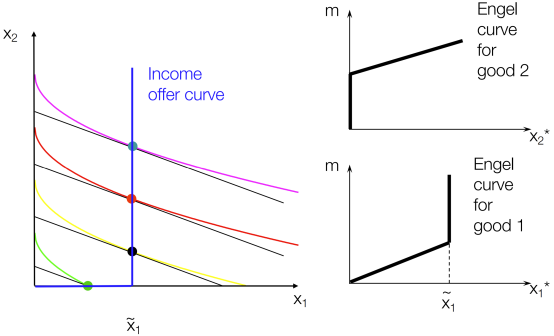
\includegraphics[width=0.5\textwidth,keepaspectratio]{preference_quasi_lineaire_expansion}
\end{figure}

\newpage
\subsection{Modification des prix}

Si on décide de fixer $p_2$ et $m$, et de modifier $p_1$ :

\subsubsection{Pour un bien ordinaire}

La demande $\nearrow$ quand son prix $\searrow$
\begin{figure}[H]
	\centering
	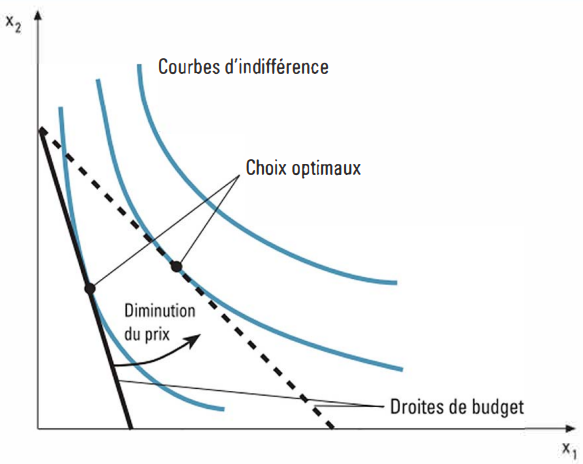
\includegraphics[width=0.5\textwidth,keepaspectratio]{diminution_bien_ordinaire}
\end{figure}


\subsubsection{Pour un bien de Giffen}

La demande $\searrow$ quand son prix $\searrow$
\begin{figure}[H]
	\centering
	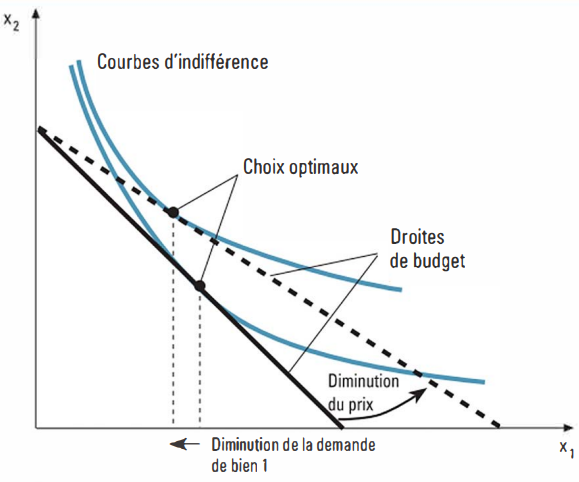
\includegraphics[width=0.5\textwidth,keepaspectratio]{diminution_bien_giffen}
\end{figure}

\newpage
\subsection{Chemin d'expansion du prix et courbe de demande}

Le prix et la quantité d'un bien varient en sens opposés : la courbe de demande a généralement une pente négative sauf pour un bien de Giffen ou la pente est positive (cas très rare).
\begin{figure}[H]
	\centering
	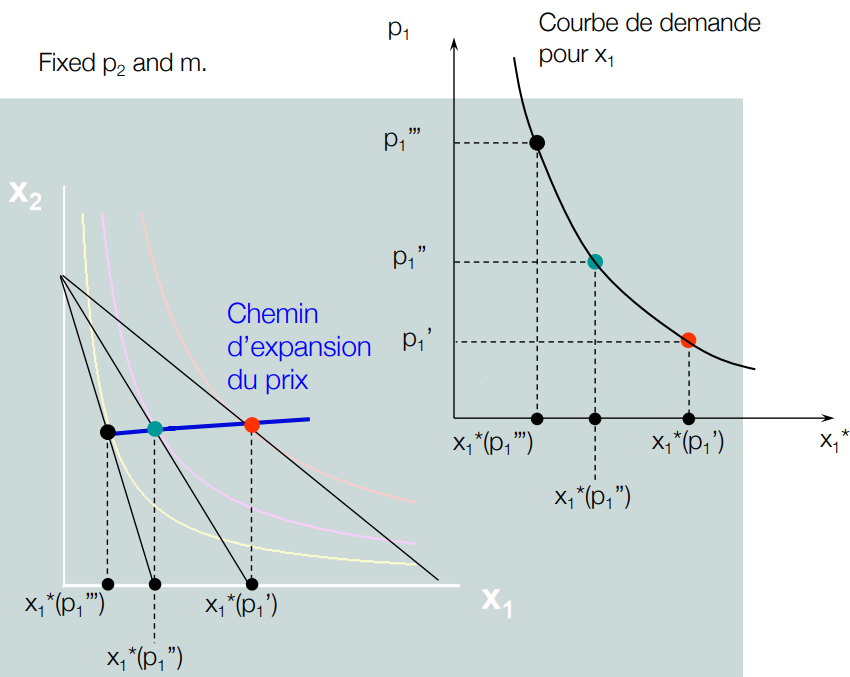
\includegraphics[width=0.5\textwidth,keepaspectratio]{chemin_expansion_courbe_demande}
\end{figure}

\subsubsection{Substituts parfaits}

\begin{figure}[H]
	\centering
	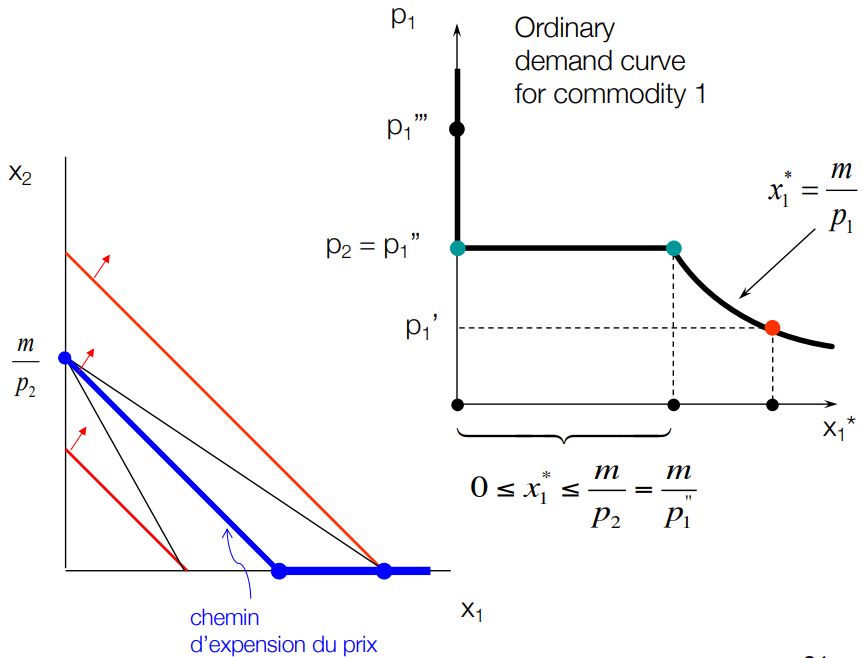
\includegraphics[width=0.4\textwidth,keepaspectratio]{chemin_expansion_courbe_demande_substituts_parfaits}
\end{figure}

\subsubsection{Compléments parfaits}

\begin{figure}[H]
	\centering
	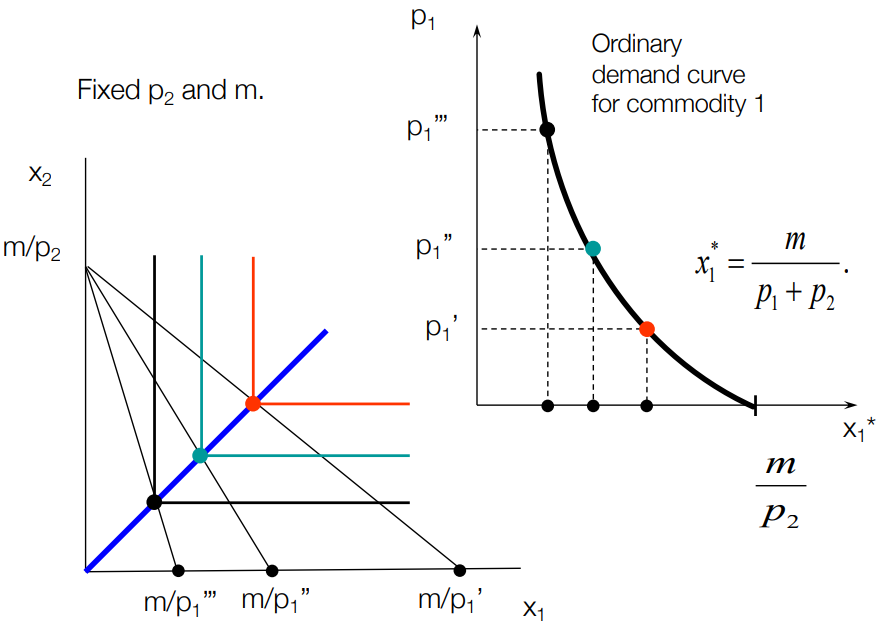
\includegraphics[width=0.4\textwidth,keepaspectratio]{chemin_expansion_courbe_demande_complements_parfaits}
\end{figure}

\subsection{Fonction de demande inverse}

Elle exprime le prix en fonction de la quantité. Pour chaque niveau de demande de bien 1, la fonction de demande inverse mesure le prix du bien 1 nécessaire pour que le consommateur choisisse ce niveau de consommation. La hauteur de la courbe de demande pour un niveau donné de consommation mesure la propension marginale à payer pour une unité additionnelle du bien à ce niveau de consommation.

\section{Évolution de la demande en fonction du prix : effet de revenu et de substitution}

But : étudier la variation d'un bien sur le choix du consommateur.

\subsection{2 effets}

\begin{itemize}
\item \textblue{Effet de substitution} : variation de la demande due à une \textred{modification du taux d'échange entre les deux bien}.
\item \textblue{Effet de revenu} : variation de la demande due à une \textred{modification du pouvoir d'achat}.
\end{itemize}

\subsection{Méthode de Slutsky}

\begin{enumerate}
\item Considérer uniquement la variation des prix relatifs en ajustant le revenu nominal pour maintenir le pouvoir d'achat constant
	\begin{itemize}
	\item[$\rightarrow$] Rotation de la droite de budget autour du panier initial $X$, la pente de la droite de budget change et on passe au panier $Y$
	\item[$\Rightarrow$] Quand le prix d'un bien décroît, nous devons diminuer le revenu de façon à maintenir le pouvoir d'achat constant.
	\end{itemize}
\item Laisser le pouvoir d'achat se modifier en maintenant les prix relatifs constants
	\begin{itemize}
	\item[$\rightarrow$] Déplacement parallèle vers le haut, la pente reste constante et c'est le pouvoir d'achat qui se modifie. On passe de $m'$ à $m$, et du panier $Y$ au panier $Z$.
	\end{itemize}
\end{enumerate}

\begin{figure}[H]
	\centering
	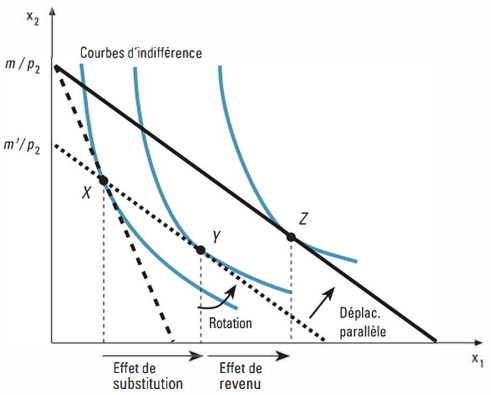
\includegraphics[width=0.4\textwidth,keepaspectratio]{slutsky}
\end{figure}


\subsection{Différents types de biens}

\subsubsection{Biens normaux}
Une diminution du revenu entraîne une diminution de la demande.
\begin{figure}[H]
	\centering
	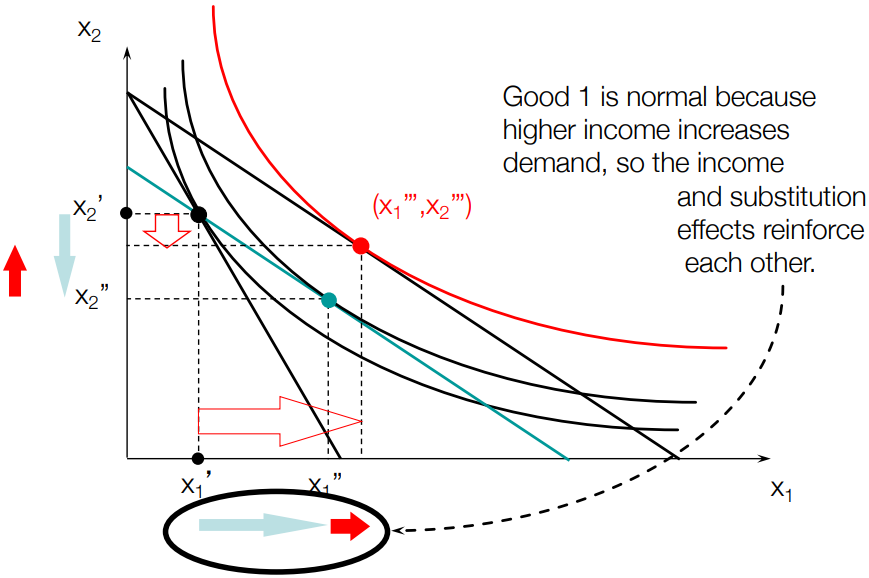
\includegraphics[width=0.4\textwidth,keepaspectratio]{slutsky_bien_normal}
\end{figure}

\newpage
\subsubsection{Biens inférieurs}
Une diminution du revenu entraîne une augmentation de la demande. les effets de substitution et de revenu s'opposent car l'effet de revenu est dans la direction opposées.
\begin{figure}[H]
	\centering
	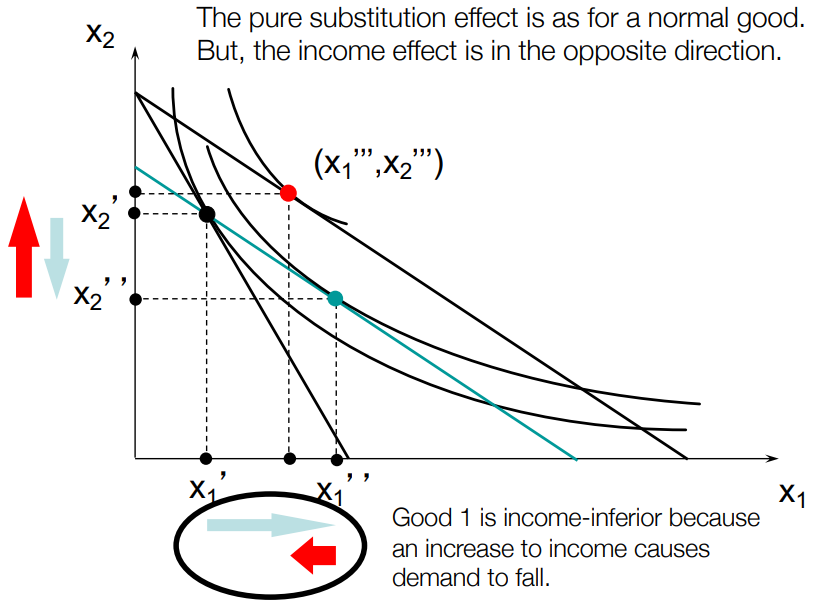
\includegraphics[width=0.4\textwidth,keepaspectratio]{slutsky_bien_inferieur}
\end{figure}

\subsubsection{Biens de Giffen}
L'effet dde revenu est supérieur à l'effet de substitution, la quantité finale demandée diminue.
\begin{figure}[H]
	\centering
	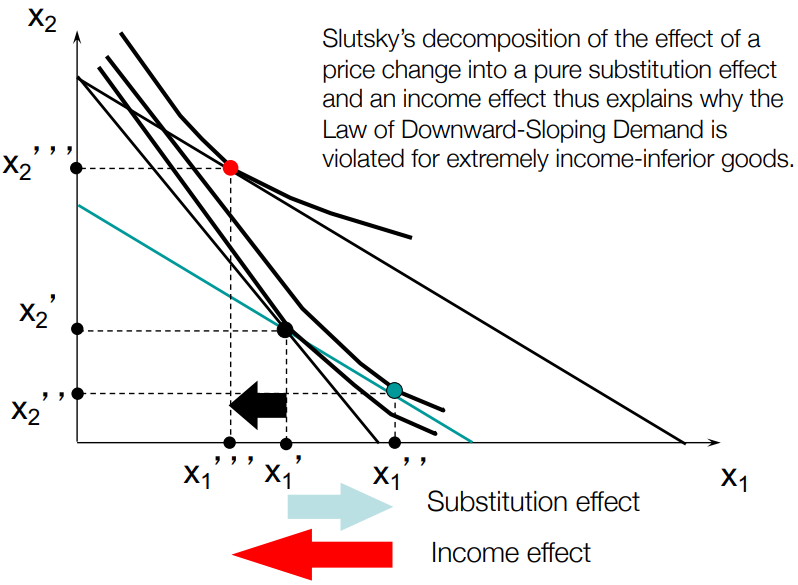
\includegraphics[width=0.4\textwidth,keepaspectratio]{slutsky_bien_giffen}
\end{figure}

\subsection{Effet de substitution de Hicks}
Supposons qu'au lieu de faire pivoter la droite de budget autour du panier initial de consommation, nus la faisions rouler le long de la CI passant par le panier initial. nous considérons ainsi un consommateur confronté à une nouvelle droite de budget finale mais à un revenu différent. le pouvoir d'achat associé à cette nouvelle droite ne permet plus d'acheter le panier initial, mais il permet d'acquérir un panier qui lui est indifférent.

\begin{figure}[H]
	\centering
	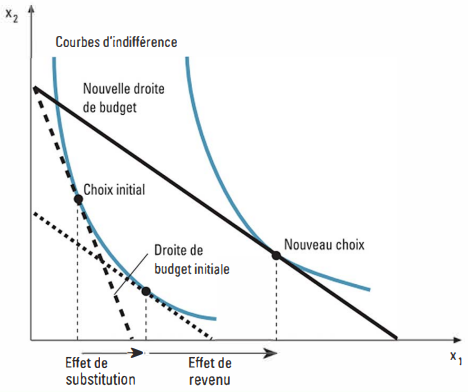
\includegraphics[width=0.4\textwidth,keepaspectratio]{substitution_hicks}
\end{figure}

\begin{enumerate}
\item Maintient l'utilité constante au lieu du pouvoir d'achat
\item \textblue{L'effet de substitution de Slutsky} donne au consommateur une somme d'argent qui lui permet de \textred{retourner à son niveau initial de consommation} alors que l'effet de substitution de Hicks lui donne une somme qui lui permet de \textred{rester sur sa CI initiale}.
\end{enumerate}

\section{L'incertitude}

il existe plusieurs états du monde possible mais l'état qui se réalisera est inconnu lors de la prise de décision $\rightarrow$ conséquences incertaines. On associe un résultat à chaque état du monde.

Ici, on suppose que l'agent économique connaît tous les états du monde possibles et la probabilité de réalisation de chacun de ces états du monde (incertitude probabilisable). Évidemment, un seul des résultats possibles va se réaliser.

\subsection{Loteries}

\begin{itemize}
\item \textblue{Manière de modéliser les actions} : choix de loteries
\item \textblue{Loterie} : distribution de probabilités sur un ensemble de résultats possibles :
\begin{equation*}
\Lagr = (\pi_1, \pi_2, ..., \pi_n|x_1, x_2, ..., x_n) \text{ où } \displaystyle\sum_{i=1}^{n} \pi_i = 1
\end{equation*}

\item \textblue{Loterie certaine} : $\Lagr = (1|x_1)$
\end{itemize}

\subsection{Préférences sur les loteries}

\begin{enumerate}
\item \textblue{Complétude} : Toute paire de loteries peut être comparée.
\item \textblue{Transitivité} : Si une loterie quelconque est au moins aussi désirable qu'une autre et cette autre au moins aussi désirable qu'une troisième, alors la première est au moins aussi désirable que la troisième.
\item \textblue{Continuité} : Aucun "petit" changement dans les probabilités n'inverse le classement entre deux loteries.
\item \textblue{Indépendance} : Si on "mélange" chaque loterie avec une troisième, alors le classement des loteries résultant ne dépend pas du choix de cette troisième loterie.
\end{enumerate}

\subsection{Utilité espérée (vNM)}

Quand l'hypothèse d'indépendance est satisfaite, on peut représenter les préférences par une fonction d'utilité particulière : la fonction d'utilité espérée ou de \textblue{von Neumann-Morgenstern}.

\begin{equation*}
U(\Lagr) = E(u(\Lagr)) = \sum_{i=1}^{n} \pi_i u(x_i)
\end{equation*}
\begin{equation*}
E(\Lagr) = \sum_{i=1}^{n} \pi_i x_i
\end{equation*}

Cette fois, la fonction d'utilité est un concept cardinal : elle permet des comparaisons de différents niveaux d'utilité. On peut maintenant dire que tel individu préfère 2x plus $L$ à $L'$.

La fonction vNM exprime le fait que la manière dont le décideur valorise la richesse dans un état du monde ne dépend pas de la manière dont il valorise la richesse dans un autre état du monde. L'individu doit choisir la meilleure loterie en fonction de ses préférences.

\newpage
\subsection{Limites : paradoxe d'Allais}

Supposons qu'il existe trois prix : 0, 500 000€ et 2 500 000€.
\begin{itemize}
\item Considérons 4 loteries portant sur ces prix dont les probabilités sont :
	\begin{align*}
	L_1 = (0, 1, 0); &L_1' = (0.1, 0, 0.9)\\
	L_2 = (0.9, 0.1, 0); &L_2' = (0.91, 0, 0.09)
	\end{align*}
\item L'individu est soumis à un choix entre $L_1$ et $L_1'$ puis entre $L_2$ et $L_2'$
\end{itemize}

\begin{minipage}{0.65\textwidth}
	La plupart préfèrent $L_1$ à $L_1'$ et $L_2'$ à $L_2$. Or, ceci est incohérent.\\
	En effet, $L_1 \succ L_1' \Leftrightarrow L_2 \succ L_2'$
\end{minipage}
\begin{minipage}{0.3\textwidth}
	\begin{figure}[H]
		\centering
		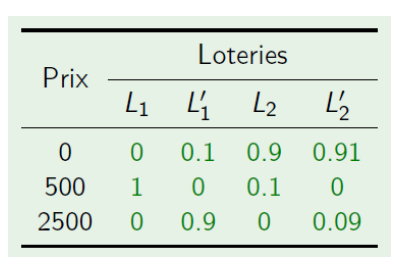
\includegraphics[width=0.7\textwidth,keepaspectratio]{paradoxe_allais}
	\end{figure}
\end{minipage}

Et :
\begin{align*}
L_1 &\succ L_1'\\
&\Leftrightarrow\\
E(U(L_1)) &> E(U(L_1'))\\
&\Leftrightarrow\\
u(500) &> 0.1u(0) + 0.9u(2500)\\
&\Leftrightarrow\\
0.1u(500) &> 0.01u(0) + 0.09u(2500)\\
&\Leftrightarrow\\
0.1u(500)+0.9u(0) &> 0.91u(0) + 0.09u(2500)\\
&\Leftrightarrow\\
E(U(L_2)) &> E(U(L_2'))\\
&\Leftrightarrow\\
L_2 &\succ L_2'
\end{align*}

\section{Aversion au risque}

\begin{itemize}
\item \textblue{Averse au risque} : Une personne manifeste de l'aversion au risque si pour tout loterie, elle trouve la loterie qui conduit certainement l'espérance de cette loterie au moins aussi désirable que la loterie elle-même. L'individu est prêt à perdre en espérance de gain pour réduire le risque auquel il est soumis.
\item \textblue{Goût pour le risque} : Si la personne préfère faiblement la loterie incertaine (>< averse).
\item \textblue{Neutre au risque} : Si la personne est indifférente entre les 2.
\item \textblue{Pari équitable} : Pari pour lequel l'espérance de gain est nul (si > 0 : plus qu'équitable).
\end{itemize}
\warning \textred{Les individus ne maximisent pas l'espérance de gain mais bien l'utilité espérée}. Le choix entre les loteries dépend de l'aversion au risque de l'agent.

Pour un individu qui manifeste de l'aversion au risque, l'utilité de la valeur attendue de la richesse, $u(10)$ = (montant initial en poche), est supérieure à son utilité attendue, $0.5u(5) + 0.5u(15)$.
\begin{figure}[H]
	\centering
	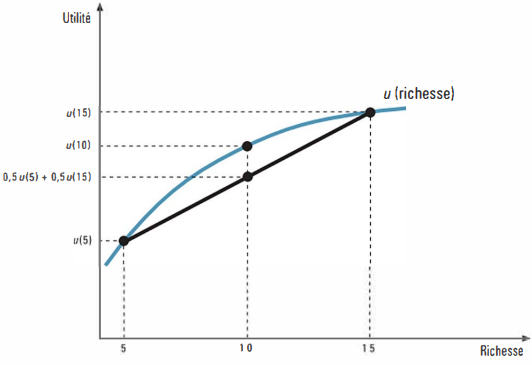
\includegraphics[width=0.4\textwidth,keepaspectratio]{aversion_risque}
\end{figure}

Pour un individu qui manifeste du goût pour le risque, l'utilité attendue de sa richesse, $0.5u(5) + 0.5u(15)$, est supérieure à l'utilité de sa valeur attendue, $u(10)$.
\begin{figure}[H]
	\centering
	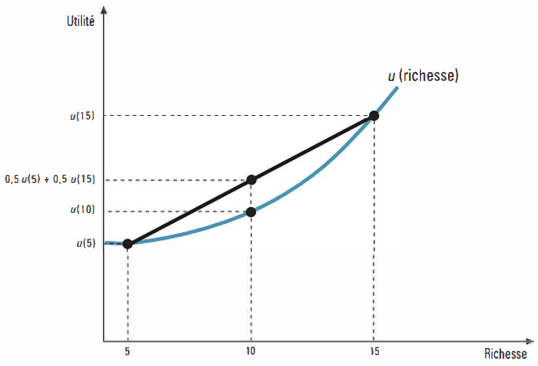
\includegraphics[width=0.4\textwidth,keepaspectratio]{gout_risque}
\end{figure}

\textit{"Winning makes you less happy than loosing makes you sad."}
\begin{itemize}
\item[$\Rightarrow$] \textblue{Aversion au risque} : fonction d'utilité \textred{strictement concave}
\item[$\Rightarrow$] \textblue{Goût pour le risque} : fonction d'utilité \textred{strictement convexe}
\item[$\Rightarrow$] \textblue{Neutre au risque} : fonction d'utilité \textred{linéaire}
\end{itemize}

\section{Choix de production}

\subsection{Technologie}

Contexte :
\begin{enumerate}
\item Une entreprise = un agent
\item Concurrence parfaite, entreprise = price taker
\item Obejctif : maximiser le profit et minimiser le coût
\end{enumerate}

Hypothèses à respecter :
\begin{enumerate}
\item \textblue{Possibilité d'inactivité} : $(0,0) \in Y$
\item \textblue{Libre disposition} : le gaspillage est toujours possible
\item \textblue{No free lunch} : impossible de produire sans input
\item \textblue{Inputs limités $\rightarrow$ output limités}
\end{enumerate}

\subsubsection{Courbes d'isoquantes}

La technologie peut être représentée par des courbes d'isoquantes. Une courbe d'isoquante est définie pour un niveau de production donné, et est le lieu des combinaisons d'inputs efficaces permettant de produire un certain niveau d'output. Elles ressembles aux Ci mais leur niveau d'utilité est déterminé par la technologie.
\begin{figure}[H]
	\centering
	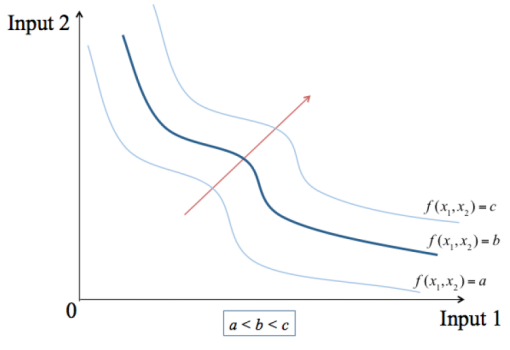
\includegraphics[width=0.4\textwidth,keepaspectratio]{isoquantes}
\end{figure}

\newpage
\subsection{Fonction de production}

\textblue{Plan de production} : Décrit l'ensemble des inputs (facteurs de production) et d'output (produits).

\textblue{Ensemble de production} : $Y$ est l'ensemble des plans de production techniquement réalisables.

\textblue{Fonction de production} : Frontière de l'ensemble de production, elle associe à chaque combinaison $x$ d'inputs données, l'output maximum $y$ qu'il est possible d'obtenir à partir de cette combinaison. C'est-à-dire : $(y_1, ..., y_m) \leq f(x_1, ..., x_n)$.

\begin{figure}[H]
	\centering
	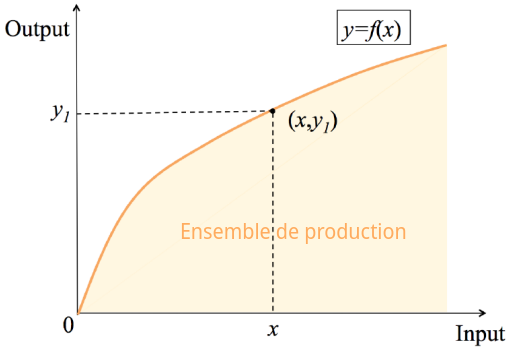
\includegraphics[width=0.3\textwidth,keepaspectratio]{fonction_production}
\end{figure}

\subsubsection{Exemples de fonctions de production}


\begin{minipage}{0.33\textwidth}
	\begin{figure}[H]
		\centering
		Substituts parfaits
		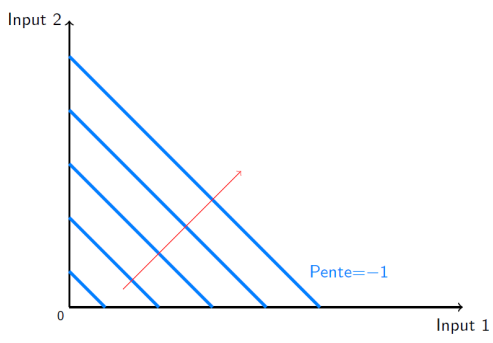
\includegraphics[width=1\textwidth,keepaspectratio]{fonction_prod_substitut}
		\legend{$f(x_1,x_2) = ax_1 + bx_2$}
	\end{figure}
\end{minipage}
\begin{minipage}{0.33\textwidth}
	\begin{figure}[H]
		\centering
		Compléments parfaits
		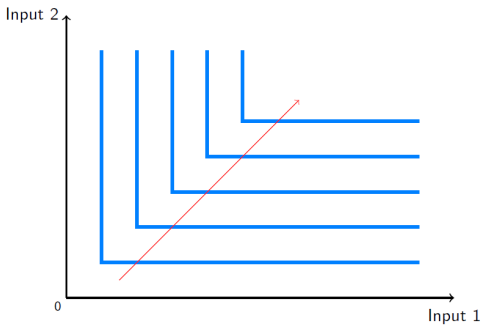
\includegraphics[width=1\textwidth,keepaspectratio]{fonction_prod_complement}
		\legend{$f(x_1,x_2) = min\{x_1, x_2\}$}
	\end{figure}
\end{minipage}
\begin{minipage}{0.33\textwidth}
	\begin{figure}[H]
		\centering
		Cobb-Douglas
		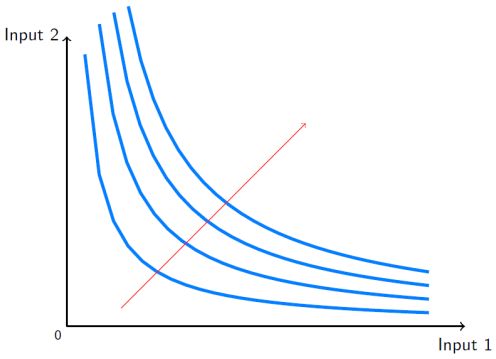
\includegraphics[width=1\textwidth,keepaspectratio]{fonction_prod_cobb_douglas}
		\legend{$f(x_1,x_2) = Ax^c_1 + x^d_2$}
	\end{figure}
\end{minipage}

\subsubsection{Hypothèses sur la fonction de production}

\begin{enumerate}
\item \textblue{Monotone} : Si on augmente la quantité d'au moins un des $x$, la quantité produite sera $>$ à celle produite initialement.
\item \textblue{Convexe} : S'il est possible de produire une certaine quantité d'$y$ de deux façons différentes, leur moyenne pondérée permet de produire une quantité $>$ de cet output.
\end{enumerate}

\subsubsection{Rendement d'échelle}

\begin{enumerate}
\item \textblue{Par rapport à la fonction de production} :\\
Pour $t > 1$ :
	\begin{itemize}
	\item Croissants : $f(tx_1, tx_2) > tf(x_1, x_2)$
	\item Décroissants : $f(tx_1, tx_2) < tf(x_1, x_2)$
	\item Constants : $f(tx_1, tx_2) = tf(x_1, x_2)$
	\end{itemize}
\item \textblue{Par rapport au produit moyen} :\\
Le produit moyen est : $PM(x) = \frac{f(x)}{x}$
	\begin{itemize}
	\item Croissants : $PM$ croissant
	\item Décroissants : $PM$ décroissant
	\item Constants : $PM$ constant
	\end{itemize}
\item \textblue{Par rapport au degré d'homogénéité} :\\
Fonction homogène de degré $k$ si $\forall(x_1, ..., x_n) et \forall t>0, f(tx_1, ..., tx_n) = t^k f(tx_1, ..., tx_n)$
	\begin{itemize}
	\item Croissants : $k > 1$
	\item Décroissants : $k < 1$
	\item Constants : $k = 0$
	\end{itemize}
\end{enumerate}

\begin{minipage}{0.33\textwidth}
	\begin{figure}[H]
		\centering
		Rendements d'échelle croissants
		~
		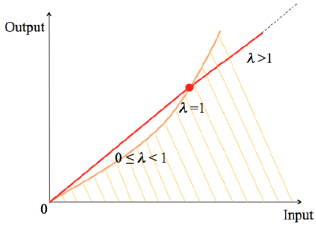
\includegraphics[width=1\textwidth,keepaspectratio]{rendement_croissant}
	\end{figure}
\end{minipage}
\begin{minipage}{0.33\textwidth}
	\begin{figure}[H]
		\centering
		Rendements d'échelle décroissants
		~
		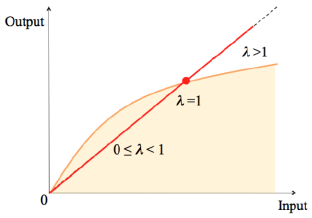
\includegraphics[width=1\textwidth,keepaspectratio]{rendement_decroissant}
	\end{figure}
\end{minipage}
\begin{minipage}{0.33\textwidth}
	\begin{figure}[H]
		\centering
		Rendement d'échelle constants
		~
		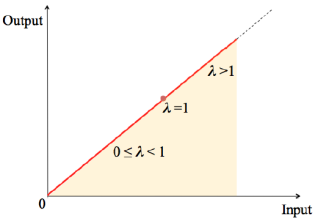
\includegraphics[width=1\textwidth,keepaspectratio]{rendement_constant}
	\end{figure}
\end{minipage}

\subsubsection{Taux marginal de substitution technique (TmST)}

Égal à la pente d'une courbe d'isoquante. il mesure comment, si la firme augmente à la marge la quantité du facteur 1, elle doit modifier la quantité du facteur 2 pour que la quantité d'output reste constante.

\begin{equation*}
TmST = - \frac{Pm_1}{Pm_2} = \text{ rapport des produits marginaux.}
\end{equation*}

\begin{figure}[H]
	\centering
	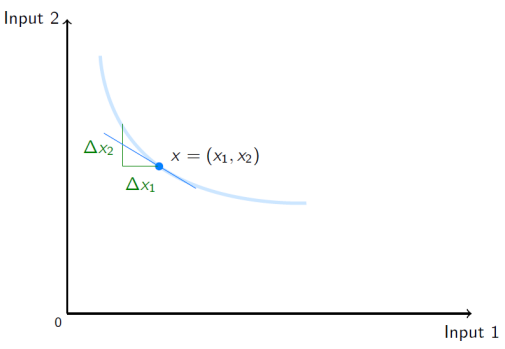
\includegraphics[width=0.4\textwidth,keepaspectratio]{tmst}
\end{figure}

\textblue{Produit marginal} : variation d'outputs par rapport à une variation unitaire du facteur $i$.
\begin{equation*}
y = f(x_1, ..., x_n) \leftrightarrow Pm_i = \frac{\partial y}{\partial x_i}
\end{equation*}

\subsection{Maximisation du profit}

\begin{enumerate}
\item Profit : Différences entre les recettes et les dépenses (les coûts) d'une entreprise $\rightarrow \pi = py - wx$
\item Recette : $py = p_1y_1, ..., p_my_m$ où $p_i$ est le prix unitaire de l'output $y_i$.
\item Dépense : $wx = w_1x_1, ..., w_n p_n$ où $w_i$ est le coût unitaire de l'input $x_i$.
\end{enumerate}

On représente le $\pi$ avec des \textred{droites s'isoprofit}. Elles regroupent l'ensemble des combinaisons d'inputs et d'outputs qui génèrent un niveau donné de profit $\{(x, y) | py - wx = \pi_0\}$.

Pour maximiser le profit, l'entreprise choisira l'ensemble de production réalisable tel que :
\begin{equation*}
\max_{x, y \in Y} \sum_{i = 1}^m p_i y_i - \sum_{j=1}^n w_j x_j \text{ s.c. } (y_1, .., y_m) \leq f(x_1, x_n)
\end{equation*}
Comme la contrainte est liante, on peut remplacer $f(x)$ dans la formule de maximisation.

\subsubsection{Maximisation à court terme}
On fixe la variable $x_2 \rightarrow \tilde{x}_2$, ce qui donne :

\begin{equation*}
\max_{x_1} p f(x_1,\tilde{x}_2) - w_1x_1 - w_2\tilde{x}_2
\end{equation*}

\newpage
La condition du choix maximale est égal à $pPm_1(x_1^*, \tilde{x}_2) = w_1$, donc la valeur du produit marginal du facteur $1$ est son prix.
\begin{figure}[H]
	\centering
	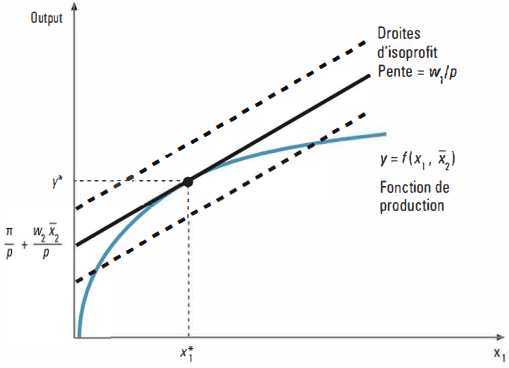
\includegraphics[width=0.35\textwidth,keepaspectratio]{maximisation_profit}
\end{figure}

\subsubsection{Maximisation à long terme}

\begin{equation*}
\max_{x_1} p f(x_1,x_2) - w_1x_1 - w_2x_2
\end{equation*}
Condition du choix optimal :
\begin{align*}
pPm_1(x_1^*, x_2^*) &= w_1\\
pPm_2(x_1^*, x_2^*) &= w_2
\end{align*}
\begin{figure}[H]
	\centering
	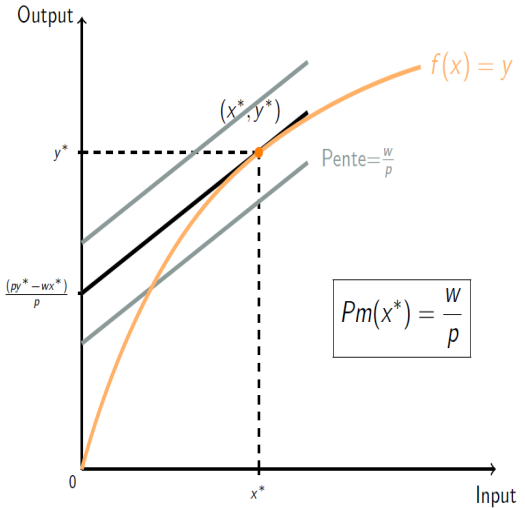
\includegraphics[width=0.3\textwidth,keepaspectratio]{maximisation_profit_long}
\end{figure}
\begin{itemize}
\item[$\rightarrow$] Similaire à la maximisation à court terme
\item[$\Rightarrow$] Égalité entre la pente des droites d'isoprofit et celle de la frontière de production.
\end{itemize}

\subsection{Minimisation du coût}

Pour décomposer le problème de maximisation :
\begin{enumerate}
\item Minimisation du coût pour produire un $y_0$ donné
\item Détermination du $y$ pour un profit maximum
\end{enumerate}

\subsubsection{Étape 1}
\begin{equation*}
\max_{x_1, x_2} w_1 x_1 + w_2 x_2 \text{ s.c. } f(x_1, x_2) = y_0
\end{equation*}

On obtient la \textred{demande conditionnelle de facteurs} :

\begin{equation*}
(x_1^*, x_2^*) = (z_1(w_1,w_2,y_0),z_2(w_1,w_2,y_0))
\end{equation*}

\textblue{Fonction de coût} : fonction associant à chaque prix des inputs les coûts minimaux de production d'un niveau donné d'outputs $y_0$. C'est une droite de pente $= -\frac{w_1}{w_2}$.
\begin{equation*}
c(w_1, w_2, y_0) = w_1x^*_1 + w_2x^*_2
\end{equation*}

\textblue{Le coût moyen} : mesure du coût minimal de production par unité d'output
\begin{equation*}
CM(w,y) = \frac{c(w_1, w_2, y_0)}{y}
\end{equation*}

\textblue{Le coût marginal} : mesure le taux de variation d'un coût minimal de production en fonction de la variation de la quantité d'output.
\begin{equation*}
Cm(w,y) = \frac{\partial c(w_1, w_2, y_0)}{\partial y}
\end{equation*}

\subsubsection{Étape 2}

\begin{equation*}
\max_y py - w_1x^*_1 + w_2x^*_2 \Longleftrightarrow \max_y py - w_1z_1(w_1,w_2,y_0) + w_2 z_2 (w_1, w_2, y_0)
\end{equation*}

On représente ce problème avec des \textred{droites d'isocoût}. Elles regroupent toutes les combinaisons d'inputs qui génèrent un niveau donné de coûts $c_0 \{(x_1, x_2)|w_1x_1 + w_2x_2 = c_0\}$.

\begin{figure}[H]
	\centering
	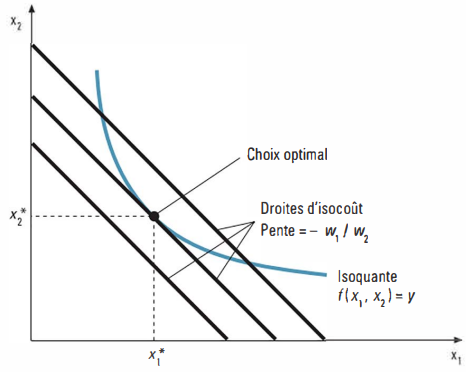
\includegraphics[width=0.3\textwidth,keepaspectratio]{minimisation_cout}
\end{figure}

\begin{itemize}
\item Trouver la droite d'isocoût la plus basse étant donné un niveau de production (courbe d'isoquante).
\item Si la fonction de production a des rendements décroissants (isoquante strictement convexe), la solution se trouve à la tangente entre la droite d'isocoût et l'isoquante.
\item $TmST = -\frac{w_1}{w_2} =$ combinaison d'inputs optimale.\\
\textit{Le choix optimal de la firme est tel que la productivité marginale de chaque output égalise son prix.}
\end{itemize}

\textblue{Rendements d'échelle} : détermine comment le coût moyen de production change avec un certain niveau d'output.
\begin{itemize}
\item Croissants : $c(ty_1, ty_2) < tc(y_1, y_2) \rightarrow$ le coût moyen diminue
\item Décroissants : $c(ty_1, ty_2) > tc(y_1, y_2) \rightarrow$ le coût moyen augmente
\item Constants : $c(ty_1, ty_2) = tc(y_1, y_2) \rightarrow$ le coût moyen ne change pas
\end{itemize}

\chapter{Partie 2}

\section{Équilibre général}

\textblue{L'équilibre général est l'étude de la fixation simultanée de tous les prix sur tous les marchés.} C'est-à-dire comment les conditions de demande et d'offre interagissent sur plusieurs marchés pour déterminer les prix de plusieurs biens.
\begin{itemize}
\item Échange pur (on considère qu'il n'y a pas de production)
\item Deux agents (A,B)
\item Deux biens (1,2)
\item Dotations (quantité disponible) : $W = (W_A, W_B) = ((w_A^1, w_A^2), (w_B^1,w_B^2))$
\item Les préférences / choix final : $X_A = (x_A^1, x_A^2)$ et $X_B = (x_B^1,x_B^2)$
\item Allocation (paire de paniers de consommation) : $X = (X_A, X_B) = ((x_A^1, x_A^2), (x_B^1,x_B^2))$
\item \textblue{Allocation réalisable} : quantité de chaque bien (allocation finale) = quantité disponible (allocation initiale)
\begin{align*}
x_A^1 + x_B^1 &= w_A^1 + w_B^1\\
x_A^2 + x_B^2 &= w_A^2 + w_B^2
\end{align*}
\end{itemize}

\subsection{Échange}

Outil de représentation : la \textblue{boite d'Edgeworth}
\begin{figure}[H]
	\centering
	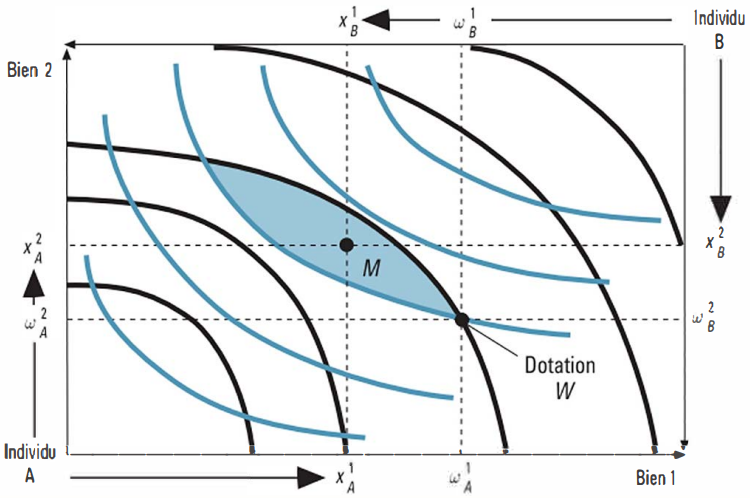
\includegraphics[width=0.5\textwidth,keepaspectratio]{boite_edgeworth}
\end{figure}

On passe de W à X : A renonce à $|x_A^1 - w_A^1|$ et reçoit $|x_A^2 + w_A^2|$ (et inversement pour B). L'intersection entre les deux zones est l'unique zone qui satisfait plus A et B que leurs dotations respectives

\subsection{Efficacité au sens de Pareto}

Une allocation est efficace au sens de Pareto s'il n'en existe pas d'autre que tous les agents préfèrent.
C'est-à-dire :
\begin{enumerate}
\item Il est impossible d'augmenter la satisfaction d'un agent sans diminuer celle d'un autre
\item Il n'y a pas de gaspillage de satisfaction
\item Tous les gains d'échange ont été exploités
\item Il n'est plus possible d'effectuer des échanges mutuellement avantageux
\end{enumerate}

Les CI doivent être tangentes pour toute allocation efficace au sens de Pareto.
\newpage
La zone où A a un niveau de satisfaction supérieur à celui de sa dotation = tous les paniers situés au-dessus de la CI passant par M. Il en est de même pour B mais de son point de vue.
\begin{figure}[H]
	\centering
	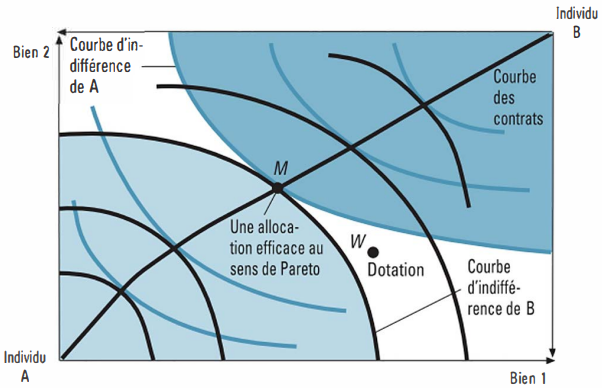
\includegraphics[width=0.5\textwidth,keepaspectratio]{allocation_pareto}
\end{figure}

\subsubsection{Ensemble de Pareto (courbe des contrats)}

Ensemble de tous les points efficaces au sens de Pareto dans une boîte d'Edgeworth.
\begin{itemize}
\item[$\rightarrow$] Tous les contrats finaux se trouvent dans cet ensemble
\item[$\rightarrow$] L'ensemble comprend toujours $O_A$ et $O_B$
\end{itemize}

\subsection{Échange marchand}

Les agents se comportent de manière concurrentielle : \textit{price takers}

\begin{itemize}
\item Le \textblue{vecteur de prix} : $(p_1,p_2)$
\item La \textblue{demande brute} : quantité totale du bien que l'agent désire $(x_A^1, x_A^2)$ et $X_B = (x_B^1,x_B^2)$
\item La \textblue{contrainte budgétaire} :
\begin{align*}
p_1 x_A^1 + p_2 x_A^2 &= p_1 w_A^1 + p_2 w_A^2\\
p_1 x_B^1 + p_2 x_B^2 &= p_1 w_B^1 + p_2 w_B^2
\end{align*}
\item La \textblue{demande nette/excédentaire} : $e_A^1 = x_A^1 - w_A^1$
\item \textblue{Marché à l'équilibre} (équilibre concurrentiel = équilibre de Walras) : ssi $e_A^1 = -e_B^1$ et $e_A^2 = -e_B^2$
\begin{itemize}
\item[$\rightarrow$] les choix de tous les consommateurs sont compatibles
\end{itemize}
\end{itemize}
\begin{figure}[H]
	\centering
	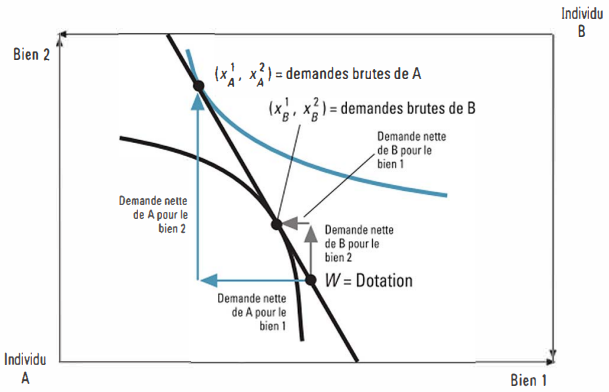
\includegraphics[width=0.48\textwidth,keepaspectratio]{demandes_bruts_nettes}\hfill
	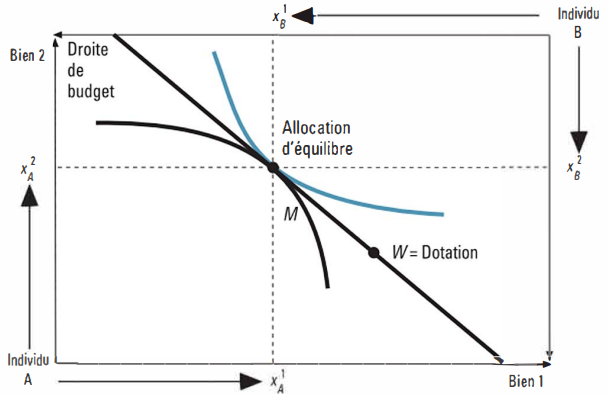
\includegraphics[width=0.48\textwidth,keepaspectratio]{equilibre_edgeworth}
\end{figure}

\subsection{Existence de l'équilibre}

Un équilibre existe sous deux conditions :
\begin{enumerate}
\item Les préférences des deux agents doivent être convexes
\item Chaque consommateur est très petit dans la population
\end{enumerate}
Grâce à ces conditions, la fonction de demande agrégée est continue $\rightarrow$ une petite variation de prix ne devrait pas entraîner un grand saut dans la quantité demandée.

\textblue{Si la fonction est continue alors un équilibre existe.}

\subsection{Efficacité de l'équilibre}

\subsubsection{Premier théorème de l'économie du bien-être}

\begin{formal}
Tout équilibre, s'il existe, est efficace au sens de Pareto
\end{formal}

$\rightarrow$ Un marché concurrentiel exploite tous les gains découlant de l'échange.

Selon la théorie des prix, les prix dirigent l'économie vers une allocation efficace. À l'équilibre compétitif, les TmS de tous les agents sont égaux et égaux au rapport des prix.

\subsubsection{Deuxième théorème du bien-être}

Inverser la causalité par rapport au théorème précédent : toute allocation efficace au sens de Pareto peut-elle être obtenue comme un équilibre compétitif (= être décentralisée) ? Oui, ssi les préférences sont convexes.
\begin{formal}
Si les préférences sont convexes, toute allocation efficace au sens de Pareto peut être décentralisée/constitue un équilibre pour un certain ensemble de prix.
\end{formal}

\section{Théorie de la justice}

\subsection{Absence d'envie - 1ère conception d'un société juste}

\subsubsection{Allocation "égalitaire"/juste/sans envie}
Allocation où les biens sont divisés de façon égale entre les agents. Il faut que $X_A \succeq_A X_B$ et que $X_B \succeq_B X_A$.

Exemple : $X_A = \frac{W}{2}$ et $X_b = \frac{W}{2} \rightarrow$ n'est pas efficace mais "égalitaire".

$\Rightarrow$ Les agents peuvent avoir des préférences différentes, ils vont donc procéder à des échanges.
\begin{formal}
Si on divise les droits de propriétés sur les ressources de manière égale entre tous les agents et qu'on laisse faire les marchés compétitifs, alors l'allocation d'équilibre sera sans envie.
\end{formal}
$\Rightarrow$ Si l'allocation initiale est divisée en parts égales, l'allocation finale doit être équitable.

Pour déterminer si une allocation est "égalitaire" ou pas, il suffit de regarder l'allocation que nous aurions si les deux agents intervertissaient leur paniers. Si cette allocation "inverse" est située en dessous des CI passant par l'allocation initiale, celle-ci est une allocation "égalitaire" ("en dessous" signifie en dessous du pont de vue de l'agent concerné; de notre point de vue, l'allocation "inverse" doit être située entre les deux CI).

\begin{figure}[H]
	\centering
	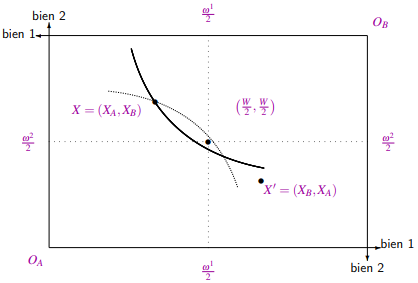
\includegraphics[width=0.5\textwidth,keepaspectratio]{allocation_sans_envie}
\end{figure}

\newpage
\subsubsection{Allocation équitable}

Allocation égalitaire et efficace au sens de Pareto.

\begin{figure}[H]
	\centering
	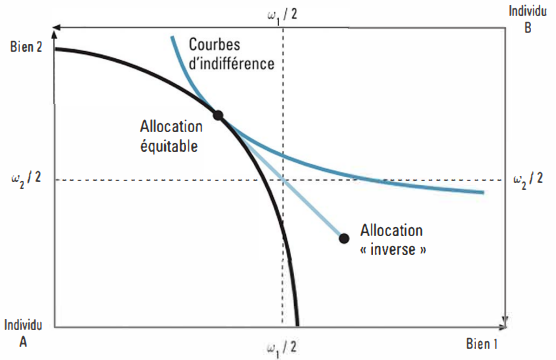
\includegraphics[width=0.5\textwidth,keepaspectratio]{allocation_equitable}
\end{figure}

\subsubsection{La conception de la justice économique comme absence d'envie}

\begin{itemize}
\item Les marchés compétitifs sont compatibles avec la justice.
\item Les conditions de la justice portent sur les droits de propriété sur les ressources (chacun une part égale).
\item Si on ajoute les firmes, on obtient le même résultat (si les droits de propriétés des firmes sont répartis de manière égale).
\end{itemize}

\subsection{Solidarité en ressources - 2ème conception d'une société juste}

\subsubsection{Solidarité en ressources}

But : garantir que tout le monde bénéficie de la croissance sans céder de l'efficacité.

\begin{figure}[H]
	\centering
	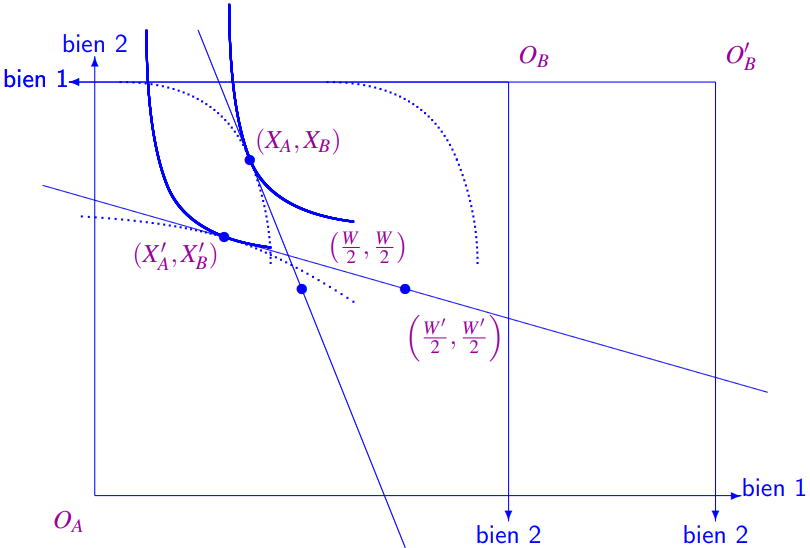
\includegraphics[width=0.5\textwidth,keepaspectratio]{solidarite_ressources}
\end{figure}

Suite à une croissance, il y a bien plus de bien 1 à allouer. Le prix du bien 1 va donc chuter. L'agent A va préférer $X_A$ à $X'_A$ car le prix du bien qu'il "vend" a baissé et celui qu'il achète a augmenter.

La croissance modifie la rareté relative des biens et cela se reflète dans les prix. Même si sa dotation augmente, l'agent A aime le bien qui est devenu le plus cher (bien 2). Il se trouve donc moins bien : $X_A \succeq_A X'_A$

$\Rightarrow$ Il est impossible de garantir la solidarité en ressource, il faut donc redistribuer.

\subsection{Conclusion}

Absence d'envie et solidarité en ressources sont 2 principes de justice incompatibles lorsqu'on joint l'efficacité. $\rightarrow$ Choisir entre les deux est un \textblue{choix éthique}.

\section{Tarification par un monopoleur}

Le vendeur est un monopoleur (= il a tous les pouvoir), l'information a donc beaucoup de valeur car elle permet à certains agents de \textblue{s'approprier une partie du surplus} qu'ils ne parviendraient pas ) avoir si l'information était complète. De plus, la manière dont l'information est distribuée influence l\textblue{a manière dont le surplus est distribué}.

Mais l'asymétrie d'information peut également impliquer une \textblue{perte de surplus total} (= diminution de l'activité économique).

\subsection{Modèle}

\begin{itemize}
\item \textblue{Bien 1} : produit par le monopoleur
\item \textblue{Bien 2} : monnaie (bien normalisé à $1$, en €)
\item \textblue{Monopoleur} :
	\begin{itemize}
	\item Produit à un coût marginal constant de $c$
	\item Propose une tarification $F$
	\item Cherche à maximiser son profit
	\end{itemize}
\item \textblue{Consommateur} :
	\begin{itemize}
	\item Le bien 1 qu'il consomme en quantité $x_1$
	\item Ce que lui coûte la transaction : $m$ (en €)
	\item Préfère un $m$ aussi petit que possible (utilité croissante en $-m$
	\end{itemize}
\end{itemize}

\subsubsection{Exemples de tarification}

\begin{itemize}
\item Prix unique : quelque soit la quantité : $F(x_1) = px_1$
\item Abonnement suivi d'un prix constant : $F(x_1) = F_0 + px_1$
\item Double prix : $p$ si $\bar{x_1} > x_1, p'$ ensuite
\item Offre à prendre ou à laisser : $(\bar{x_1}, F(\bar{x_1})$
\item Un seuil : $x_1$
\end{itemize}

\subsubsection{Fonction d'utilité du consommateur}

\begin{equation*}
U(x_1, -m) = \textblue{v(x_1)} \textred{-m}
\end{equation*}

Elle est quasi-linéaire : linéaire en \textred{monnaie}, non linéaire en \textblue{biens}.

\subsubsection{Surplus du consommateur}

C'est ce qu'il gagne en bien être dans la transactions.

La fonction $v(x)$ représente le surplus d'utilité que le consommateur tire de la consommation du bien.
\begin{itemize}
\item Elle est concave : volonté à payer décroissante
\item Elle est croissante : volonté à payer toujours positive
\end{itemize}
$v(x) =$ l'utilité marginale (elle est toujours positive, et sa dérivée est toujours négative).

\subsubsection{Maximisation de l'utilité}

Le consommateur fait face à une tarification $F$. \textblue{Contrainte} : la quantité d'argent que le consommateur va débourser doit être supérieure ou égale à la quantité d'argent que le vendeur demande.
\begin{equation*}
\max_{x_1, -m} U(x_1, -m) \text{ s.c. } m \geq F(x_1)
\end{equation*}
Comme la contrainte doit être liante, on a :
\begin{equation*}
\max_{x_1, -m} U(x_1, -m) = v(x_1) - F(x_1)
\end{equation*}
Le maximum est atteint lorsque la dérivée première est nulle
\begin{equation*}
\frac{d v(x_1^*)}{dx_1} = \frac{dF(x_1^*}{dx_1}
\end{equation*}
$\Rightarrow$ Le résultat est le même en cas de bons d'achat (car $B$ est une constante qui disparaît en dérivant) : la quantité optimale dépend uniquement de $v$ et $F$.

\subsubsection{Propriétés des fonctions d'utilité quasi-linéaires}

\begin{enumerate}
\item L'effet revenu est nul
\item La demande du consommateur est insensible à l'augmentation du revenu : le bien 1 doit être très petit dans le budget du consommateur
\item Le surplus du consommateur peut se mesurer en monnaie
\item Richesse nette = richesse brute - coût de production
\end{enumerate}
Les CI sont parallèles entre elles, et l'utilité se mesure sur l'axe horizontal (donc en €)

\begin{figure}[H]
	\centering
	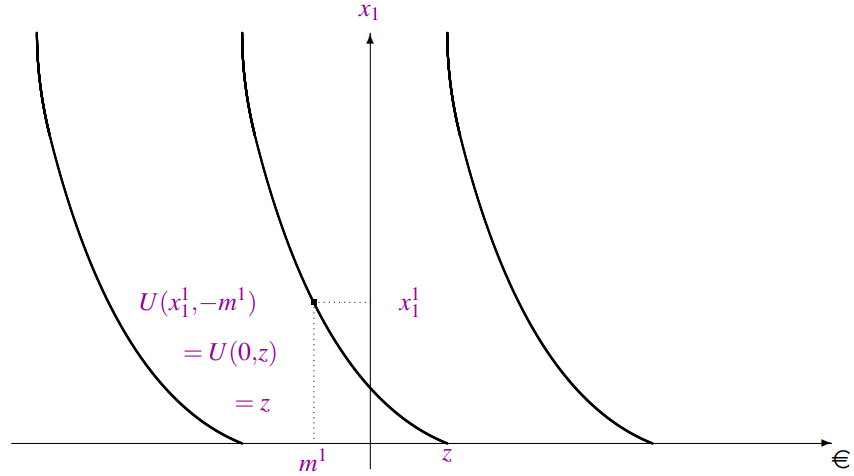
\includegraphics[width=0.5\textwidth,keepaspectratio]{tarification_monopoleur}
\end{figure}

\subsubsection{Rappel sur le Lagrangien}

\begin{equation*}
\max f(x) \text{ s.c. } g(x) \geq b
\end{equation*}
\begin{enumerate}
\item On ajoute une nouvelle variable : "le multiplicateur de Lagrange"
	\begin{equation*}
	\max \Lagr = f(x) \textred{-} \lambda (\textred{b - g(x)})
	\end{equation*}
	\textred{Membre de la parenthèse} : On écrit la contrainte sous la forme "$... < 0$"
\item On dérive le Lagrangien selon toutes ses variables
	\begin{equation*}
	f'(x) = + \lambda^* g'(x) = 0
	\end{equation*}
	\begin{itemize}
	\item Si $\lambda^* < 0$ : \textred{impossible}
	\item Si $\lambda^* = 0$ : $g(x) > b$
	\item Si $\lambda^* > 0$ : $g(x) = b$ (contrainte liante)
	\end{itemize}
\end{enumerate}

\subsection{Un consommateur, un producteur et un planificateur}

\textblue{Planificateur} : bienveillant et omniscient (il dispose de 100\% de l'information). Il décide de la quantité à produire et de la manière de répartir le surplus entre le consommateur et le producteur.
$\Rightarrow$ s'il veut garantir un profit $\bar{\Pi}$ au producteur :
\begin{equation*}
\max_{x_1, F} U(x_1, -F) = v(x_1) - F \text{ s.c. } F - c x_1 \geq \bar{\Pi}
\end{equation*}

\begin{enumerate}
\item Le Lagrangien s'écrit : $\Lagr = v(x_1) - F - \lambda(\bar{\Pi} - (F - c x_1))$
\item La solution : dériver par rapport aux "vraies" variables :
	\begin{enumerate}
	\item[] $\frac{\partial \Lagr}{\partial x_1} = v'(x_1) - \lambda c = 0 \Leftrightarrow v'(x^*_1) = c$
	\item[] $\frac{\partial \Lagr}{\partial F} = - 1 + \lambda = 0 \Leftrightarrow \lambda = 1$ ($\lambda > 0$, la contrainte et bien liante)
	\end{enumerate}
\item On obtient donc : $\frac{\partial \Lagr}{\partial \lambda} = -(\bar{\Pi} - (F - cx_1)) = 0$
\end{enumerate}
$\Rightarrow$ Comme la contrainte est liante, $F - c x_1 = \bar{\Pi}$.
La quantité produite ($v(x_1) - c x_1$) est celle qui maximise le surplus.
\begin{figure}[H]
	\centering
	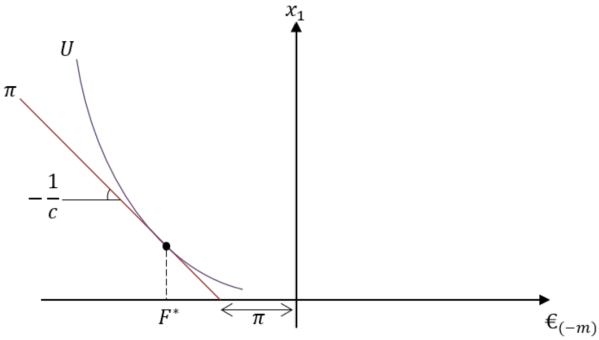
\includegraphics[width=0.5\textwidth,keepaspectratio]{planificateur}
\end{figure}
\begin{itemize}
\item[$\Rightarrow$] Au plus la droite se déplace vers la gauche, au plus $\pi$ augmente
\item[$\rightarrow$] Le \textit{producteur} voit son utilité \textit{augmenter} si on se déplace vers la gauche
\item[$\rightarrow$] Le \textit{consommateur} voit son utilité \textit{diminuer} si on se déplace vers la gauche
\end{itemize}

\subsection{Un consommateur et un monopoleur en information parfaite}

\subsubsection{Contrainte de participation du consommateur}

\begin{equation*}
U(x_1, -m) \geq U(0,0) \Leftrightarrow v(x_1) - m \geq 0
\end{equation*}

\textblue{Le monopoleur choisira la tarification qui maximise son profit}. $m = F$, donc ce que dépense le consommateur est ce que reçoit le monopoleur.

\subsubsection{Objectif du monopoleur}

\begin{equation*}
\max_{x_1, F} F - c x_1 \text{ s.c. } v(x_1) - F \geq 0
\end{equation*}

\begin{enumerate}
\item Le Lagrangien s'écrit : $\Lagr = F - c x_1 - \lambda (F - v(x_1))$
\item La solution : dériver par rapport aux "vraies" variables :
	\begin{enumerate}
	\item[] $\frac{\partial \Lagr}{\partial x_1} = - c + \lambda v'(x_1) = 0 \Leftrightarrow v'(x^*_1) = c$
	\item[] $\frac{\partial \Lagr}{\partial F} = 1 - \lambda = 0 \Leftrightarrow \lambda = 1$ ($\lambda > 0$, la contrainte et bien liante)
	\end{enumerate}
\item Comme la contrainte est liante, on a : $F^* = v(x^*_1)$, et comme $F = m$, on obtient : $U(x^*_1, F^*) = 0 \rightarrow$ le consommateur est donc indifférent entre acheter et ne pas acheter.
\end{enumerate}

\textblue{La solution est efficace} car tout le surplus potentiel est réalisé. \textblue{Le monopoleur accapare tout le surplus}.\\
$\rightarrow$ Plusieurs tarifications différentes peuvent mener à la même solution dont une tarification avec un abonnement et un prix constant $c$ ou un contrat à prendre ou à laisser $(x^*_1, F^*)$.
\begin{figure}[H]
	\centering
	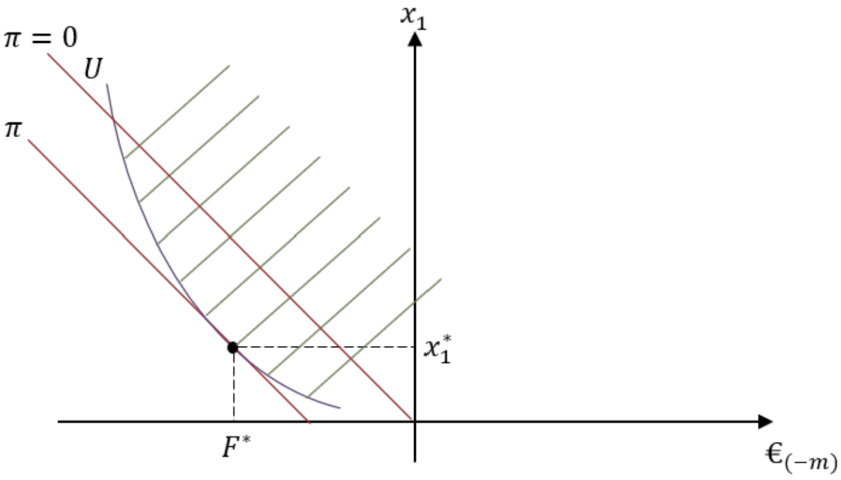
\includegraphics[width=0.5\textwidth,keepaspectratio]{cons_mono}
\end{figure}
$\Rightarrow$ Le consommateur accepte tous les contrats situés dans la zone hachurée en vert.

\subsection{Plusieurs consommateurs et un monopoleur en information parfaite}

Information complète = monopoleur omniscient.
Il y a deux types de consommateurs qu'on peut ordonner en fonction de leur goût pour le bien 1.

\begin{equation*}
U(x_1, -m) = g v(x_1) - m \text{ s.c. } g_a > g_b
\end{equation*}

$\rightarrow$ La volonté à payer de $a$ est toujours supérieure à celle de $b$. Le profit sera donc toujours plus élevé en échangeant avec $a$.

\subsubsection{Condition de single crossing}
\begin{itemize}
\item Les CI des deux agents aux goûts différents se croisent au plus une fois
\item Tous les consommateurs peuvent être rangés selon une seule dimension
\item Le TmS d'un consommateur de type $a$ est en tout point supérieur à celui d'un autre consommateur de type $b$.
\end{itemize}
\begin{figure}[H]
	\centering
	\includegraphics[width=0.4\textwidth,keepaspectratio]{p_cons_mono}
\end{figure}
Le monopoleur peut donc proposer 2 contrats différents $(x^*_a, F^*_a)$ et $(x^*_b, F^*_b)$ aux 2 types d'agents comme s'il faisait affaire avec séparément.\\
$\rightarrow$ Répliquer la solution précédente.\\
\textblue{La solution est efficace} car tout les surplus potentiel est réalisé. \textblue{Le monopoleur accapare tout le surplus}.\\
$\rightarrow$ Plusieurs tarifications différentes peuvent mener à la même solution dont une tarification avec un abonnement avec un prix contrant $p$ = $c$ ou une double tarification à prendre ou à laisser.\\
$\Rightarrow$ \textblue{Solution optimale de premier rang}

\subsection{Plusieurs consommateurs et un monopoleur en information incomplète}

Monopoleur incapable de distinguer les agents de types $a$ et $b$ mais connaît la probabilité de faire face à chaque type. Il est donc en situation d'incertitude.\\
\warning Cas d'antisélection : un consommateur de type $a$ peut se faire passer pour un consommateur de type $b$ (et inversement).\\
Le monopoleur se limite aux offres à prendre ou à laisser et on suppose qu'il est neutre au risque.

\begin{equation*}
\Pi = q_a(F^i_a - c x^i_a) + q_b(F^i_a - c x^i_a)
\end{equation*}
Avec $q_a$ et $q_b$ les probabilités de faire face à un agent de type $a$/$b$.

\subsubsection{Contraintes de participation (CP)}

\begin{itemize}
\item $U_a(x^i_a, F^i_a) = g_a v(x^i_a - F^i_a)$
\item $U_b(x^i_b, F^i_b) = g_b v(x^i_b - F^i_b)$
\end{itemize}

\subsubsection{Contraintes de compatibilité avec les incitants (CI)}

Il faut tenir compte du fait qu'un type de consommateur pourrait avoir envie de se faire passer pour l'autre
\begin{itemize}
\item $U_a(x^i_a, F^i_a) \geq U_a(x^i_b, F^i_b)$
\item $U_b(x^i_b, F^i_b) \geq U_b(x^i_a, F^i_a)$
\end{itemize}

\subsubsection{Simplification des contraintes}

Sachant que $g_a > g_b$ : $U_a(x^i_a, F^i_a) \geq U_a(x^i_b, F^i_b) \geq U_b(x^i_b, F^i_b) \geq 0$

La CP de $a$ est donc satisfaite. Les agents $a$ peuvent avoir intérêt à se faire passer pour un agent $b$ mais pas le contraire.

\begin{equation*}
\max_{x_1, F} q_a(F_a^i - c x_a^i) + q_b (F_b^i - c x_b^i) \text{ s.c. } U_b(x^i_b, F^i_b) \geq 0 \text{ et } U_a(x^i_a, F^i_a) \geq U_a(x^i_b, F^i_b)
\end{equation*}

Par l'hypothèse de single corssing, $g_a > g_b$. Il y a trois cas à analyser :

\begin{enumerate}
\item Les volontés à payer des deux types d'agents sont supérieures à $c$
\begin{figure}[H]
	\centering
	\includegraphics[width=0.3\textwidth,keepaspectratio]{agents_sup_c}
\end{figure}
Le contrat $D$ n'est pas optimal ($a$ choisira toujours un contrat dans la zone hachurée au lieu de $D$).

\item Les volontés à payer des deux types d’agents sont inférieures à $c$
\begin{figure}[H]
	\centering
	\includegraphics[width=0.3\textwidth,keepaspectratio]{agents_inf_c}
\end{figure}
Le contrat $D$ n’est pas optimal ($b$ choisira toujours un contrat dans la zone hachurée au lieu de $D$).

\item La volonté à payer de $a$ est supérieure à $c$ et la volonté à payer de $b$ est inférieure à $c$
\begin{figure}[H]
	\centering
	\includegraphics[width=0.3\textwidth,keepaspectratio]{a_b_c}
\end{figure}
Le contrat $D$ n’est pas optimal ($a$ et $b$ choisiront toujours un contrat dans une des zones hachurées au lieu de $D$)
\end{enumerate}

$\Rightarrow$ Proposer uniquement le contrat $D$ ne sera jamais optimal pour le monopoleur car le contrat ne peut être mélangeant. Il faut qu'l propose \textblue{autant de contrats qu'il y a de types de consommateurs}.

\subsubsection{Solution optimale}

Le monopoleur doit modifier sa politique : diminuer $x^i_b$ et donc son $F$ associé (il prélève ainsi moins de surplus sur les agents $b$). En faisant cela, il diminue l'envie qu'ont les agents $a$ de se faire passer pour les agents $b$.

\begin{enumerate}
\item[$\rightarrow$] Il peut donc augmenter le prix payé par les agents $a$ et accaparer une plus grande part de leur surplus
\item[$\rightarrow$] Il y a autant de contrats que d'agents
\item[$\rightarrow$] L'équilibre est séparant (information révélée post transaction)
\end{enumerate}
\begin{figure}[H]
	\centering
	\includegraphics[width=0.4\textwidth,keepaspectratio]{solution_optimale}
\end{figure}

\subsubsection{Agents de type a}

\begin{itemize}
\item Quantité achetée = celle achetée en information complète
\item Montant payé < celui payé en information complète
	\begin{itemize}
	\item[$\Rightarrow$] Strictement mieux qu'en information complète grâce à une rente informationnelle
	\end{itemize}
\end{itemize}

\subsubsection{Agents de type b}

\begin{itemize}
\item Quantité achetée < celle achetée en information complète (demande volontairement distordue par le monopoleur)
\item Montant payé < celui payé en information complète
	\begin{itemize}
	\item[$\Rightarrow$] Utilité pas affectée par l’asymétrie d’information
	\end{itemize}
\end{itemize}

$\Rightarrow$ \textblue{Le surplus total est moindre} qu'en information complète
\textblue{Solution optimale de second rang} : activité économique et bien-être créé < solution de premier rang mais cette dernière est inaccessible.

\subsection{Concurrence parfaite}

Si les firmes sont présentes en très grande nombre, elles deviennent des prices takers et doivent fixer leur prix à $p = c$. Il n'y a plus de distortion.\\
Les agents choisissent librement leurs quantités, donc :
\begin{enumerate}
\item L'agent $a$ demandera $x_a^*$ au prix $cx_a^*$ pour maximiser $U_a = g_av(x_a) - cx_a$
\item L'agent $b$ demandera $x_b^*$ au prix $cx_b^*$ pour maximiser $U_b = g_bv(x_b) - cx_b$
\end{enumerate}

L'équilibre est efficace au sens de Pareto et le surplus est alors maximal mais, cette fois-ci, il est accaparé intégralement par les consommateurs $\rightarrow$ la distribution de l'information est devenue non-pertinente.
